% Variance de l'estimateur d'une pente en fonction de la corrélation entre les deux
% régresseurs : V[b̂₁] = σ²/(T(1-ρ²)), tracée ici pour σ² = 1 et deux tailles
% d'échantillon.
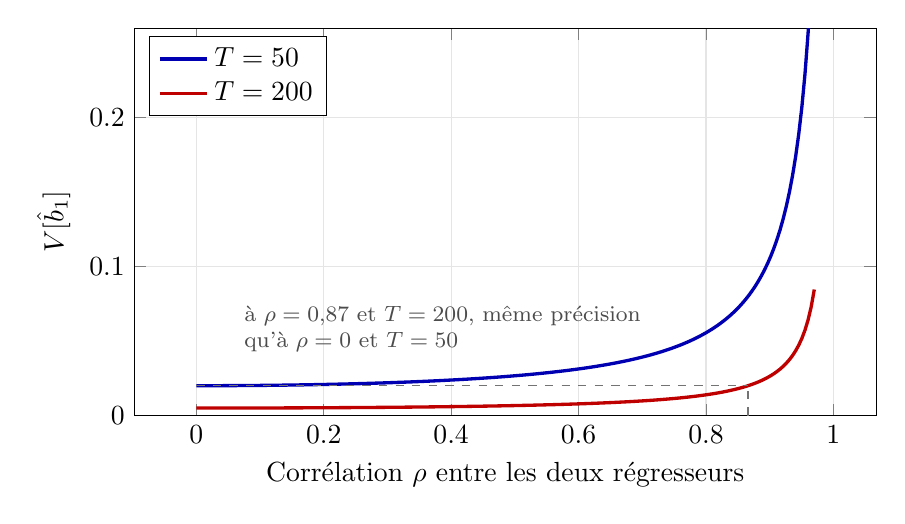
\begin{tikzpicture}[
    declare function={variance(\r,\t) = 1/(\t*(1-\r*\r));}
]
\begin{axis}[
  width = 11cm, height = 6.5cm,
  xlabel = {Corrélation $\rho$ entre les deux régresseurs},
  ylabel = {$\mathbb V[\hat b_1]$},
  samples = 200,
  domain = 0:0.97,
  ymin = 0, ymax = 0.26,
  legend cell align = left,
  legend style = {at={(0.02,0.98)}, anchor=north west},
  grid = major, grid style = {gray!20}]

  \addplot[very thick, blue!70!black, mark={}] {variance(x,50)};
  \addlegendentry{$T = 50$}

  \addplot[very thick, red!75!black, mark={}] {variance(x,200)};
  \addlegendentry{$T = 200$}

  % À précision égale, quadrupler l'échantillon permet de tolérer ρ = 0,866.
  \draw[dashed, black!55] (axis cs:0,0.02) -- (axis cs:0.866,0.02);
  \draw[dashed, black!55] (axis cs:0.866,0) -- (axis cs:0.866,0.02);
  \node[anchor=west, font=\footnotesize, black!70, align=left] at (axis cs:0.06,0.058)
       {à $\rho=0{,}87$ et $T=200$, même précision\\ qu'à $\rho=0$ et $T=50$};
  \node[anchor=north, font=\footnotesize, black!70] at (axis cs:0.866,-0.004) {$0{,}87$};

\end{axis}
\end{tikzpicture}
